\documentclass{article}
\usepackage[utf8]{inputenc}
\usepackage{graphicx}
\usepackage{fourier}
\usepackage{multicol}

\begin{document}

\title{Preload-dependent power laws in detachment dynamics of probabilistic fasteners}
\author{}
\date{}
\maketitle

Before detachment from an elastic fabric substrate occurs, mushroom arrays do not in general
follow a linear force-strain relationship characterized by the ``per mushroom'' modulus $E$.
The non-linearity of the force response as the mushrooms load the fibers is apparent in 
the raw force-distance curves presented in Figure \ref{fig:f_d}. For preloads that exceed 20 N,
there in no single slope that characterises the curves in the stage following the preload, but
before the detachment process.

\begin{figure}
    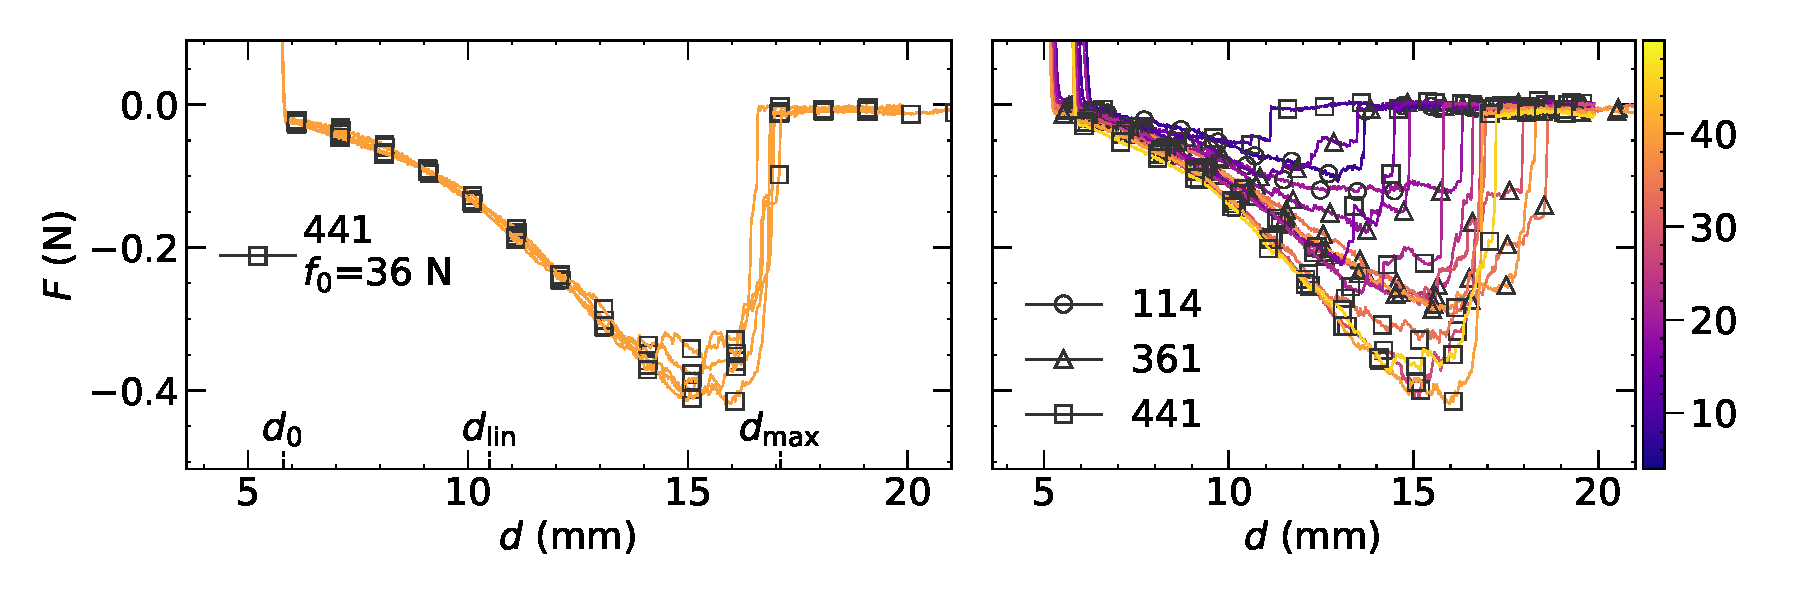
\includegraphics[width=0.9\linewidth]{f_d.pdf}
    \caption{Raw force-distance curves of mushroom-patterned silicone rubber adhesive pads
    detaching from a textile substrate consisting of nylon fibers. \label{fig:f_d}}
\end{figure}

The non-linearity of the loading regime represents a preliminary challenge to the validity
of fibre bundle models, which attempt to capture the microscopic features of the 
feature-fabric interaction. In a basic form, such a model would feature a linear loading
regime $F=E\lambda$, followed by a failure regime $\exp{(-\frac{E\lambda}{\sigma_0})^m}$,
with the latter term representing the survival probability of a feature at strain $\lambda$.
Since our curves disobey linearity at low $\lambda$, we need to, first, explain the 
non-linearity, and, second, present a modified model.

An intuitively appealing explanation is the notion of \textit{activation} -- in the initial
loading, the textile fibers are not stretched, and as such do not carry load. In other words,
the initial deformation is ``for free''. We attempted to model activation by dividing the force
by an activity coefficient $\xi=(1-\exp{-\frac{\lambda}{\lambda_m}})^{-1}$. By the strain $\lambda$ 
we under the non-dimensionalised gap size after correcting for the zero-force ``loading'' point 
$\lambda=\frac{d-d_0}{d_\mathrm{max}}$ and by $\lambda_m$ is meant $\frac{L_m}{d_\mathrm{max}}$. $L_m$ must
then be a constant independent from preload and feature density, varied over a conservative
range from 114 to 441 features per 25$\cdot$25 mm$^2$. The presumed role of $L_m$
as a geometric parameter is required by the fact that fibers are assumed to attach 
to only one feature, as such being unable to perceive the mushroom densities. 

We do not find evidence for the validity of activation in our data: from the fact that 
some force-distance curves \textit{are} actually linear at low strain, it should be 
clear that we can not expect one $L_m$ to take care of reducing all loading regimes
to a linear load line. Thus, we attempted to collapse the data by varying $L_m$ between
50 $\mu$m to 5 mm to achieve collapse. However, Figure \ref{fig:inact_domain}, in which we 
multiply the $x$-axis by $\xi$, shows that even an activation parameter optimized \textit{per curve}
does not result in a model that describes the loading process. 

\begin{figure}
    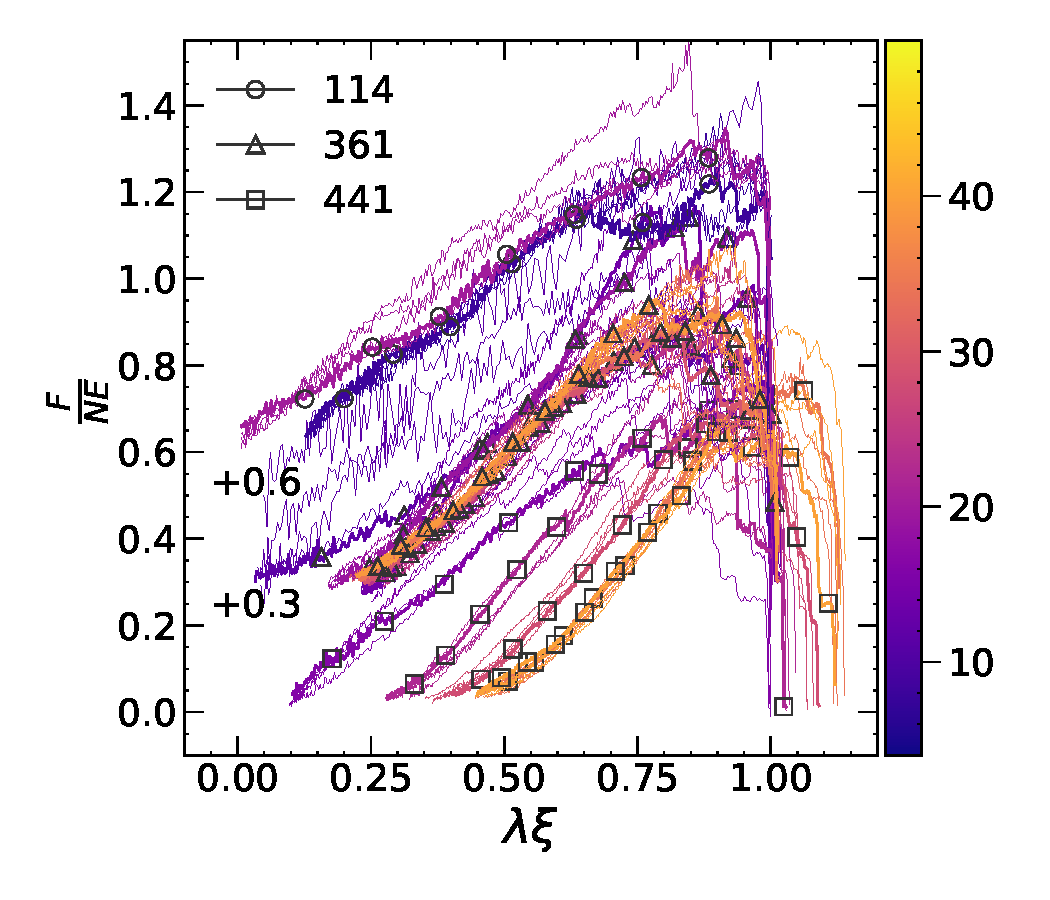
\includegraphics[width=0.9\linewidth]{inact_domain.pdf}
    \caption{Force-distance curves taken from Figure \ref{fig:f_d} converted to force-activated strain
    curves. Strain is multiplied by the activation coefficient $\xi$. Force is normalized by
    $E$, which is the average slope obtained from linear regression of the unnormalized force-strain curves.
    \label{fig:inact_domain}}
\end{figure}

Rather, the fiber stretching imposes a power law on the force-distance curve, which
we show in Figure \ref{fig:logforce} as a straight line through on a plot of $\log \frac{f}{NA}$
against $\log \lambda$.  

\begin{figure}
    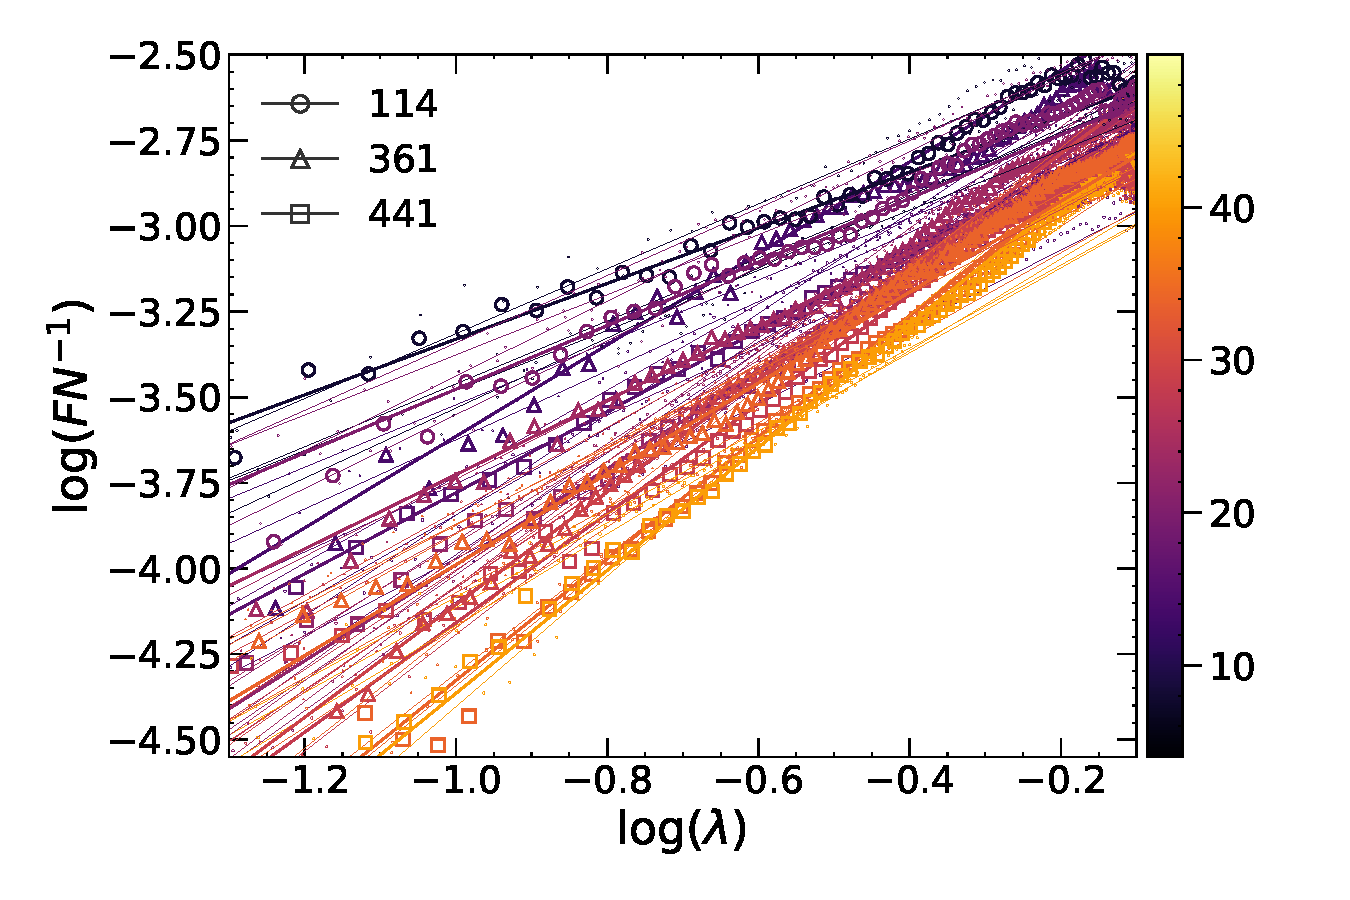
\includegraphics[width=0.9\linewidth]{sigma_powerlaw.pdf}
    \caption{Log(force)-low(strain) curves with straight lines found with linear regression.\label{fig:logforce}}
\end{figure}

Subsequently, we re-fit all curves in Figure \ref{fig:inact_domain} to an equation which combines
a power law loading regime, followed by the aforementioned probabilistic decay factor:

\begin{figure}
    \label{fig:powerbull}
    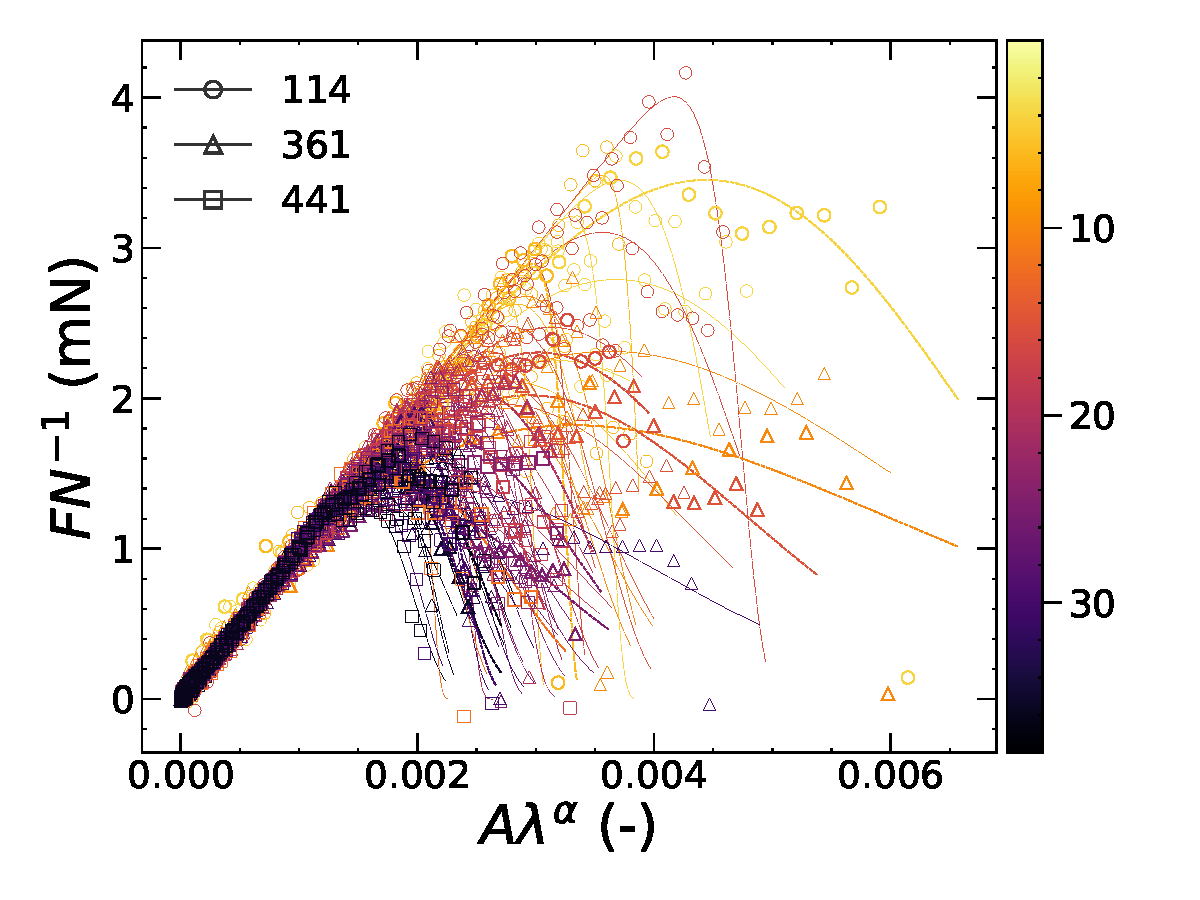
\includegraphics[width=0.9\linewidth]{powerbull_collapse.pdf}
    \caption{Fits of force-strain curves to Equation \ref{eq:powerbull}. The loading regime
    is successfully collapsed by inserting the power law $\lambda^\alpha$.}
\end{figure}


\begin{equation}
    \label{eq:powerbull}
    FN^{-1}=A\lambda^\alpha\exp{-(\frac{E\lambda}{\sigma_0}^m)}
\end{equation}

Good fits to the data were accomplished with least squares optimization. We used the
powers and pre-factors from Figure \ref{fig:logforce} to initialize the fits, and $\sigma_0$ 
and $m$ were initialized with linear regression on one representative curve using a linearised
version of Equation \ref{eq:powerbull} with $\alpha=1$, which was sufficient to find 
reasonable values for all curves. $E$ was left fixed.  Figure \ref{fig:powerbull} shows that fits
describe the loading regime excellently. 

The failure regime of arrays with small $N~1\cdot10^2$ can not reasonably expected to follow
$\exp{-(\frac{E\lambda}{\sigma_0}^m)}$, since the latter factor assumes a continues distribution 
of critical failure stresses, which requires $N \to \infty$. A result is a dramatic overestimation
of $m$: we fit values as high as 20. 

A surprising result of the present analysis is that power law $\alpha$ varies between 
1 and $\frac{3}{2}$, as seen in Figure \ref{fig:fitpars}. We analyze the emergence 
of a power law with strength $\frac{3}{2}$ as strain hardening caused by the presence of
entanglements between the fibers (``crosslinks''). Stretching of the fibers causes
a concomitant tensing-up at the intersection points, resulting in a progressively 
stiff network of fibers as more strain is applied. The dependence of the power on preload
can be seen as the presence of a critical active fiber density beneath which the formation
of intersection points is unlikely. At low densities, we simply measure the (linear, at all
low strains) elasticity of the nylon strands.

We note that strain hardening with a power law of
strength $\frac{3}{2}$ is a common feature seen in crosslinked polymer networks of semi-flexible 
polymers. \textit{Yes, I will put the citation here.}

\begin{figure}
    \label{fig:fitpars}
    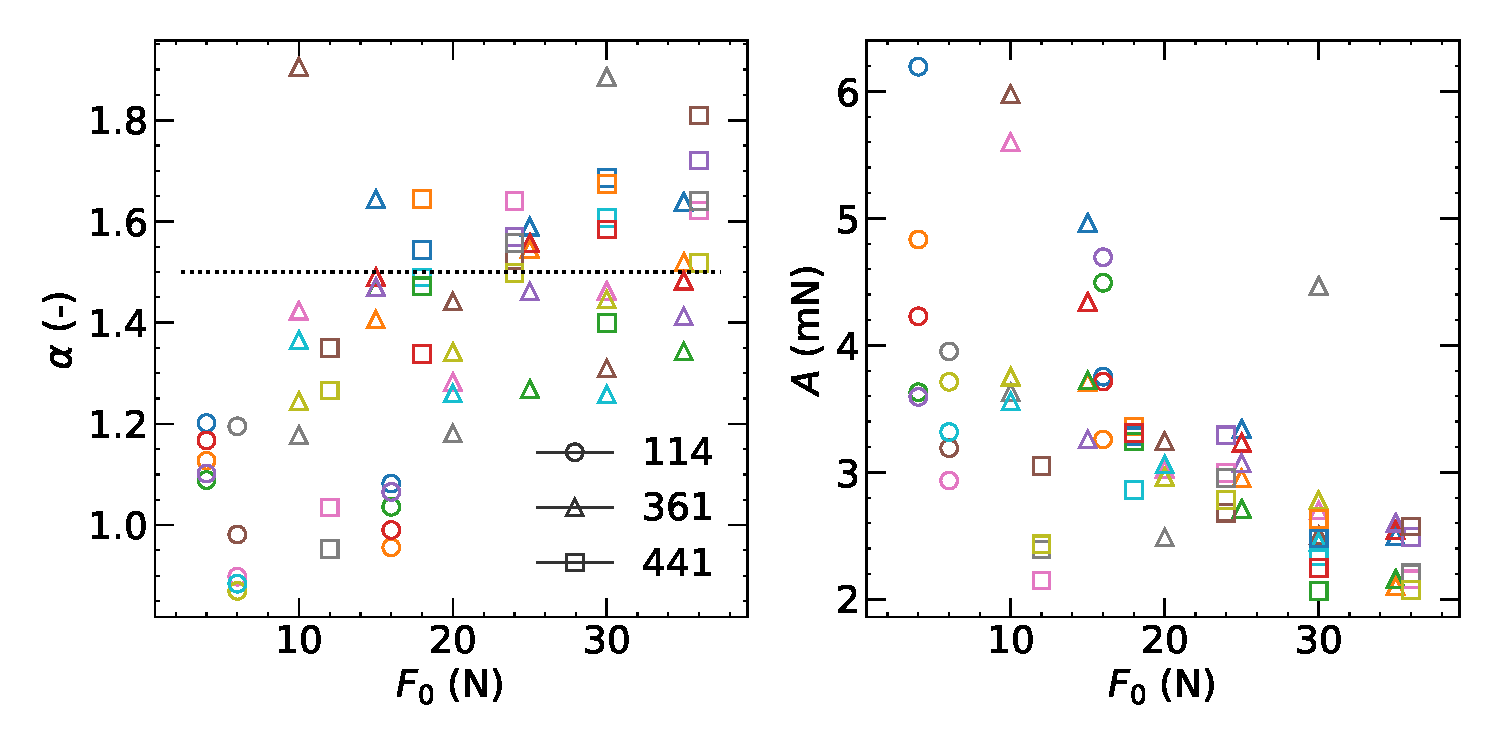
\includegraphics[width=0.9\linewidth]{powerbull_2panel.pdf}
    \caption{Fit parameters $\alpha$ and $A$ as functions of preload $F_0$ as obtained from
    least squares optimization of force-strain data to Equation \ref{eq:powerbull}. The horizontal
    dashed line indicates the value $\frac{3}{2}$.}
\end{figure}




\end{document}
